%%%%%%%%%%%%%%%%%%%%%%%%%%%%%%%%%%%%%%%%%%%%%%%%%%%%%%%%%%%%%%%%%%%%%%%%%%%%%%%%
%%%%%%%%%%%%%%%%%%   Vorlage für eine Abschlussarbeit   %%%%%%%%%%%%%%%%%%%%%%%%
%%%%%%%%%%%%%%%%%%%%%%%%%%%%%%%%%%%%%%%%%%%%%%%%%%%%%%%%%%%%%%%%%%%%%%%%%%%%%%%%

% Erstellt von Maximilian Nöthe, <maximilian.noethe@tu-dortmund.de>
% ausgelegt für lualatex und Biblatex mit biber

% Kompilieren mit
% lualatex dateiname.tex
% biber dateiname.bcf
% lualatex dateiname.tex
% lualatex dateiname.tex
% oder einfach mit:
% make

\documentclass[
  12pt,
  tucolor,
  BCOR=15mm,     % 12mm binding corrections, adjust to fit your binding
  % parskip=half,  % new paragraphs start with half line vertical space
  open=any,      % chapters start on both odd and even pages
  cleardoublepage=plain,  % no header/footer on blank pages
]{tudothesis}

\usepackage{geometry}
\geometry{a4paper, margin=2.5cm, top=3.5cm}
\renewcommand{\baselinestretch}{1.5}

% Warning, if another latex run is needed
\usepackage[aux]{rerunfilecheck}

% just list chapters and sections in the toc, not subsections or smaller
\setcounter{tocdepth}{1}

% change spacing before chapters
\RedeclareSectionCommand[beforeskip=30pt]{chapter}

%------------------------------------------------------------------------------
%------------------------------ Sprache und Schrift: --------------------------
%------------------------------------------------------------------------------
\usepackage{fontspec}
\defaultfontfeatures{Ligatures=TeX}  % -- becomes en-dash etc.

% german language
\usepackage{polyglossia}
\setdefaultlanguage{german}

% for english abstract and english titles in the toc
\setotherlanguages{english}

% intelligent quotation marks, language and nesting sensitive
\usepackage[autostyle]{csquotes}

% microtypographical features, makes the text look nicer on the small scale
\usepackage{microtype}

%------------------------------------------------------------------------------
%------------------------ Für die Matheumgebung--------------------------------
%------------------------------------------------------------------------------

\usepackage{amsmath}
\usepackage{amssymb}
\usepackage{mathtools}

% Enable Unicode-Math and follow the ISO-Standards for typesetting math
\usepackage[
  math-style=ISO,
  bold-style=ISO,
  sans-style=italic,
  nabla=upright,
  partial=upright,
]{unicode-math}
\setmathfont{Latin Modern Math}

% nice, small fracs for the text with \sfrac{}{}
\usepackage{xfrac}


%------------------------------------------------------------------------------
%---------------------------- Numbers and Units -------------------------------
%------------------------------------------------------------------------------

\usepackage[
  locale=DE,
  separate-uncertainty=true,
  per-mode=symbol-or-fraction,
]{siunitx}
\sisetup{math-micro=\text{µ},text-micro=µ}

%------------------------------------------------------------------------------
%-------------------------------- tables  -------------------------------------
%------------------------------------------------------------------------------

\usepackage{booktabs}       % stellt \toprule, \midrule, \bottomrule

%------------------------------------------------------------------------------
%-------------------------------- graphics -------------------------------------
%------------------------------------------------------------------------------

\usepackage{graphicx}
\usepackage{grffile}
\usepackage{subcaption}

% allow figures to be placed in the running text by default:
\usepackage{scrhack}
\usepackage{float}
\floatplacement{figure}{htbp}
\floatplacement{table}{htbp}

% keep figures and tables in the section
\usepackage[section, below]{placeins}


%------------------------------------------------------------------------------
%---------------------- customize list environments ---------------------------
%------------------------------------------------------------------------------

\usepackage{enumitem}

%------------------------------------------------------------------------------
%------------------------------ Bibliographie ---------------------------------
%------------------------------------------------------------------------------

\usepackage[
  backend=biber,   % use modern biber backend
  autolang=hyphen, % load hyphenation rules for if language of bibentry is not
                   % german, has to be loaded with \setotherlanguages
                   % in the references.bib use langid={en} for english sources
]{biblatex}
\addbibresource{references.bib}  % die Bibliographie einbinden
\DefineBibliographyStrings{german}{andothers = {{et\,al\adddot}}}

\usepackage[labelformat=simple]{subcaption}
\renewcommand\thesubfigure{(\alph{subfigure})}

%------------------------------------------------------------------------------
%------------------------------ Sonstiges: ------------------------------------
%------------------------------------------------------------------------------

\usepackage[pdfusetitle,unicode,linkbordercolor=tugreen]{hyperref}
\usepackage{bookmark}
\usepackage[shortcuts]{extdash}

%------------------------------------------------------------------------------
%-------------------------    Angaben zur Arbeit   ----------------------------
%------------------------------------------------------------------------------

\author{\underline{Kevin Sedlaczek}\\ Björn Wendland}
\title{Klassifizierung von Erkrankungen der menschlichen Iris mit Methoden des maschinellen Lernens auf Bildern Optischer Kohärenztomographie}
\date{\today}
% \birthplace{Castrop-Rauxel}
\chair{Lehrstuhl für Experimentelle Physik IV / V}
\division{Fakultät Physik}
\thesisclass{Projektbericht zum Seminar \textit{Maschinelles Lernen für Physikstudierende}}
% \submissiondate{31. Juli 2018}
% \firstcorrector{Dr.~Johannes Erdmann}
% \secondcorrector{Dr.~Olaf Nackenhorst}

% tu logo on top of the titlepage
\titlehead{
\includegraphics[height=1.5cm]{logos/tu-logo.pdf}}

\begin{document}
\frontmatter
% \thispagestyle{empty}
\setcounter{page}{2}
\section*{Hinweise}
Empfohlen wird die Verwendung dieser Vorlage mit der jeweils aktuellsten TeXLive Version (Linux, Windows) bzw. MacTeX Version (MacOS).
Aktuell ist dies TeXLive 2016. Download hier:
\begin{center}
  \ttfamily\url{https://www.tug.org/texlive/}
\end{center}
Bei Verwendung von TexLive Versionen 2014 und älter sollte
die Zeile
\begin{center}
\verb+\RequirePackage{fixltx2e}+ 
\end{center}
als erste Zeile der Präambel noch vor der Dokumentenklasse eingefügt werden.
Dies lädt diverse Bugfixes für LaTeX, die ab TexLive 2015 Standard sind.

Die Vorlage \texttt{thesis.tex} ist für die Kompilierung mit \texttt{lualatex} ausgelegt, mit wenigen Anpassungen kann sie aber auch mit \texttt{pdflatex} oder \texttt{xelatex} verwendet werden. 
Die Dokumentenklasse \texttt{tudothesis.cls} kann mit allen drei Programmen verwednet werden.

Achten Sie auch auf die Kodierung der Quelldateien.
Bei Verwendung von Xe\LaTeX\ oder Lua\LaTeX\ (empfohlen) müssen die
Quelldateien UTF-8 kodiert sein.
Bei Verwendung von pdf\LaTeX\ nutzen Sie die Pakete \texttt{inputenc} und \texttt{fontenc} mit der korrekten Wahl der Kodierungen.

Eine aktuelle Version dieser Vorlage steht unter 
\begin{center}
  \ttfamily\url{https://github.com/maxnoe/tudothesis}
\end{center}
zur Verfügung.

Alle verwendeten Pakete werden im \LaTeX{} Kurs von Pep et al.\ erklärt:
\begin{center}
  \ttfamily\url{http://toolbox.pep-dortmund.org/notes}
\end{center}

Für Rückmeldungen und bei Problemen mit der Klasse oder Vorlage, bitte ein \emph{Issue} auf GitHub aufmachen oder eine Email an
\href{mailto:maximilian.noethe@tu-dortmund.de}{maximilian.noethe@tu-dortmund.de} schreiben.

Wenn Sie die Dokumentenklasse mit der Option \texttt{tucolor} laden, werden verschiedene Elemente in TU-Grün gesetzt.

\maketitle

% Gutachterseite
% \makecorrectorpage

% hier beginnt der Vorspann, nummeriert in römischen Zahlen
% \thispagestyle{plain}

\section*{Kurzfassung}
Hier steht eine Kurzfassung der Arbeit in deutscher Sprache inklusive der Zusammenfassung der
Ergebnisse.
Zusammen mit der englischen Zusammenfassung muss sie auf diese Seite passen.

\section*{Abstract}
\begin{english}
The abstract is a short summary of the thesis in English, together with the German summary it has to fit on this page.
\end{english}

\tableofcontents

\mainmatter
% Hier beginnt der Inhalt mit Seite 1 in arabischen Ziffern
\chapter{Problemstellung und Datensatz}

Das Feld des Maschinellen Lernens (ML) ist seit einiger Zeit eines der sich
schnell entwickelnden und immer stärker viele praktische Anwendungen liefernden
Gebiete. Nicht nur in der Wissenschaft werden die Möglichkeiten dieser Methoden
immer stärker genutzt. Auch in vielen anderen Gebieten wird von Bild- und
Spracherkennung, Datenanalyse und Vorhersage bis hin zu medizinischen Diagnosen
profitiert. Die Methoden des maschinellen Lernens ermöglichen viele bisher nicht
da gewesene Automatisierungen und computerbasierte Verfahren. \\
Dazu gehören viele Probleme, die für Menschen schwierig zu lösen sind, aber in
ihrer Art sehr gut geeignet für Maschinen, da sie sich gut Formalisieren lassen.
Allerdings gibt es genau so auch Aufgaben, die für menschliche Intelligenz sehr
intuitiv und effizient lösbar sind, Maschinen allerdings vor große
Herausforderungen stellen. Dazu gehören Probleme wie das Erkennen von Sprache
oder das Klassifizieren von Bildern.
Hierbei können bestimmte Arten neuronaler Netze sehr effektiv Ergebnisse
liefern.
In dieser Arbeit werden die Ergebnisse eines ML-Ansatzes zur Erkennung von
Erkrankungen der menschlichen Iris anhand medizinischer Bildgebungsverfahren
diskutiert.

\section{Problemstellung}

Die optische Kohärenztomograhpie (OCT) ist ein weit verbreitetes optische
Bildgebungsverfahren, welches zum Beispiel in der Medizin Verwendung
findet. Es kann dazu verwendet werden, nicht-invasiv hochauflösende
Bilder des Querschnitts einer menschlichen Retina an lebenden Patienten
zu erstellen.\\
Diese dienen erfahrenen Ärzten dazu frühzeitig Erkrankungen zu erkennen
und so die richtigen Diagnosen zu stellen. Da das Erstellen solcher Bilder
und die Diagnose anhand dieser die Zeit eines erfahrenen Arztes benötigt
und viele Millionen solcher Bilder jährlich anfallen, ist die Suche nach
einer automatisierten Diagnose bereits aus wirtschaftlicher Sicht sinnvoll.
Außerdem lässt sich auch die Frage stellen, ob Verfahren des ML vielleicht
sogar eine bessere Genauigkeit bei der Klassifizierung der Krankheiten erreichen
können, als Ärzte.\\
Aus dieser Motivation heraus beschäftigt sich diese Arbeut mit der folgenden
Problemstellung.\\
\newline
\noindent\fbox{%
    \parbox{\textwidth}{%
        \centering
        \textbf{Mit welcher Genauigkeit lassen sich Erkrankungen der menschlichen Iris
        anhand von Aufnahmen mittels optischer Kohärenztomograhpie mit Methoden
        des maschinellen Lernens klassifizieren?}
    }%
}\\

\section{Datensatz}
%
Der dazu verwendete Datensatz stammt von der Webseite \textit{kaggle}, welche
viele Datensätze aus dem Gebiet der \textit{data science} zur Verfügung stellt.
Er stammt aus einer Veröffentlichung \cite{paper}, welche sich mit derselben
Fragestellung befasst, wie die in dieser Arbeit diskutierten. \\
Der Datensatz ist unter der \textit{Creative Commons} Lizenz
\texttt{CC BY-NC-SA 4.0} veröffentlicht und enthält $84\,495$ Bilder im
JPEG-Format. Diese sind jeweils etwa $500\text{px}\times500\text{px}$ groß
und repräsentieren OCT-Aufnahmen von 4 Klassen:
%
\begin{itemize}
  \item NORMAL: gesunde Augen
  \item CNV (\textit{Choroidal Neovascularization}): Flüssigkeitseinlagerungen unterhalb der Retina
  \item DME (\textit{Diabetic Macular Edema}): Verdickungen der Retina in Verbindung mit Flüssigkeitseinlagerungen in der Retina
  \item DRUSEN (\textit{Multiple Drusen}): Drusen unterhalb der Retina
\end{itemize}
%
Die Aufnahmen für die einzelnen Klassen sind beispielhaft in
Abbildung~\ref{fig:scans} dargestellt.
%
\begin{figure}
  \centering
  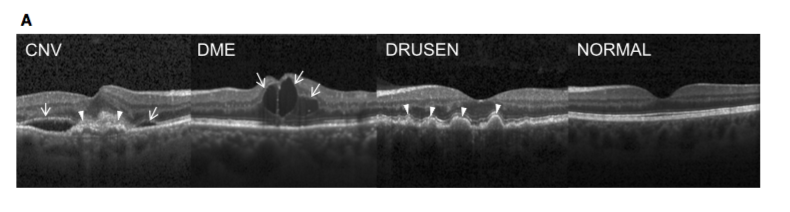
\includegraphics[width=1.1\textwidth]{Plots/title.png}
  \caption{Beispiele für die OCT Aufnahmen der 4 Klassen.}
  \label{fig:scans}
\end{figure}
%
Es handelt sich um schwarz-weiße Bilder unterschiedlicher Größen. Es fällt auch
auf, dass die Ausrichtungen der einzelnen Bilder variieren. Um eine problemfreie
Verarbeitung der Daten zu gewährleisten, werden diese daher zunächst auf eine
Größe von $400\text{px}\times400\text{px}$ vereinheitlicht. Dies bedeutet also
je nach Ausgangsbild den Verlust oder das Auffüllen von Pixeln. Die Grauwerte
der Bilder werden für das Training auf einen Zahlenwert im Intervall $[0,\,1]$
skaliert.

{\let\clearpage\relax \chapter{Convolutional Neural Networks}\label{sec:netze}}

Zur Klassifizierung von Bildern haben sich in der Vergangenheit so genannte
\textit{Convolutional Neural Networks} (CNN) als sehr effektiv bewiesen \cite{goodfellow}.
Diese wenden, wie im Namen impliziert, die mathematische Operation der Faltung
(oder in den meisten Fällen der Kreuzkorrelation) zwischen mindestens zwei
\textit{layern} des Netzes an.
Dazu wird ein Kernel definiert, welcher deutlich kleiner als die Eingabe ist.
Dieser Kernel rastert die Eingabe ab und erzeugt dabei die Ausgabe lokal auf
kleineren subsamples der Eingabe. Dabei wird also ein set linearer Aktivierungen
erzeugt.
Diese speziellen neuronalen Netze unterscheiden sich von herkömmlichen Netzen
allgemein in 3 Punkten:
%
\begin{enumerate}
  \item \textbf{Wechselwirkungen}: Anstatt wie bei vollständig vernetzten
  Netzen durch eine einfache Matrixmultiplikation alle Knoten zwischen zwei
  Lagen wechselwirken zu lassen, werden durch kleine Kernelgrößen
  Eigenschaften auf deutlich kleineren subsamples der Eingabe bestimmt. Dies dient
  z.B. der Erkennung von Strukturen und Eigenschaften der zu erkennenden Klassen.
  \item \textbf{Parameter}: In herkömmlichen Netzen werden die vom Netz
  generierten Gewichte exakt einmal genutzt, nämlich wenn die Ausgabe der
  besagten Lage generiert wird. CNN hingegen teilen sich diese Parameter mit
  verschiedenen Knoten. Gewichte eines Knotens sind also an Gewichte eines
  Anderen gebunden, da derselbe Kernel überall angewandt wird.
  \item \textbf{Equivarainz}: Die Struktur von CNN verleiht diesen eine
  Eigenschaft, die Equivarainz genannt wird. Das heißt, dass sich
  Verschiebungen der Eingabe genauso in der Ausgabe widerspiegeln. Dies ermöglicht
  CNN, bestimmte Eigenschaften in z.B. einem Bild an verschiedenen Orten zu erkennen
  und deren Gewichte zu teilen.
\end{enumerate}
%
Diese Unterschiede stellen bereits deutlich heraus, was CNN so geeignet für die
Erkennung von Bildern macht. Die Verbindung von mehreren Faltungslagen
ermöglicht so die sukzessive Erkennung von Strukturen in Bildern. \\
Typisch für Netze mit der Aufgabe der Bilderkennung ist also eine oben
beschriebene Faltungsoperation, gefolgt von einer nichtlinearen Aktivierung.
Der Output dieser Faltungslagen wird in einem zweiten Schritt in einem so
genannten \textbf{pooling layer} (PL) verarbeitet. Dieser nimmt im Prinzip eine
Vergröberung vor. Der hier verwendete \textit{max pooling layer} z.B. ersetzt
die Eingabe in einem bestimmten, kleinen Bereich durch das Maximum. So wird das
Gelernte unabhängiger von kleinen Änderungen gemacht, da die Ausgabe des PL sich
unter kleinen Verschiebungen der Eingabe nur geringfügig ändern. Dieser Schritt
stellt eine wichtige Komponente eines funktionierenden Netzes dar, wenn es
nicht nur wichtig ist, wo sich ein bestimmtes Merkmal befindet, sondern
\textit{ob} es sich in dem Bild befindet.
Außerdem spielen PL eine wichtige Rolle bei der Verarbeitung von Daten
variabler Dimension.

\section{Hauptarchitektur des CNN}
%
Die Netzarchitektur, die sich im Laufe dieser Arbeit als die Effektivste
herausgestellt hat (i.F. Hauptarchitektur), ist in Tabelle~\ref{tab:haupt} dargestellt. Es hat
sich im Laufe der Bearbeitung zunächst herausgestellt, dass die Kombination
aus \texttt{Conv2D} Lage und \texttt{MaxPooling} Lage eine gut
funktionierende Grundlage für das vorliegende Problem ist.
Daher besitzt die Hauptarchitektur zwei Einheiten dieser Kombination
direkt zu Beginn des Netzes. Hier soll also die Zerlegung der Bilder auf
die in Abschnitt~\ref{sec:netze} beschriebene Weise stattfinden.
Die beiden \texttt{Conv2D} Lagen rastern das Bild über einen $4\times4$
Kernel ab. Daher entstehen die in Tabelle~\ref{tab:haupt} aufgeführten
Dimensionen. Das Bild wird mit $(2, 2)$ \textit{strides} durchfahren,
sodass sich die Dimension des Bildes von $400\times400$ zunächst auf
$199\times199$ reduziert. Eine \texttt{MaxPooling} Lage reduziert diese
mit $(3, 3)$ \textit{strides} auf $66\times66$. Die folgende Einheit
aus  \texttt{Conv2D} und \texttt{MaxPooling} Lage lieferen schließlich
einen Output der Dimension $10\times10$.\\
Dieser Output wird schließlich in den vollständig vernetzten Teil des
Netzes gespeist. Hierbei hat sich gezeigt, dass sowohl eine kleine Anzahl
Filter in der Größenordnung $64$ als auch eine sehr große Zahl der
Größenordnung $1000$ die Leistung des Netzes verringern. Bei einer sehr großen
Anzahl an Filtern in den Dichtelagen liegt der überwiegende Teil der
trainierbaren Parameter in einer Dichtelage. Diese Übergewichtung einer Lage
wird mit kleineren Dichtelagen verhindert. Außerdem reduziert sich so die
Gesamtgröße des Netzes, was sich signifikant in der Rechenzeit niederschlägt.
Daher sind hier fünf Dichtelagen mit den angegeben Größen implementiert.
Die Anzahl der Dichtelagen wurde dabei lediglich händisch variiert und das
beste Ergebnis gewählt.
%
\begin{table}[htb]
  \centering%
  \begin{tabular}{l
                  l
                  l}
      \toprule
      Layer (type)    & Output Shape     & Anzahl Parameter      \\
      \midrule
      Conv 2D         & (199, 199, 64)  & 1\,088 \\
      Max Pooling 2D  & (66, 66, 64)    & 0 \\
      Conv 2D         & (32, 32, 32)    & 32\,800 \\
      Max Pooling 2D  & (10, 10, 32)    & 0 \\
      Dropout (0,25)  & (10, 10, 32)    & 0 \\
      Dense           & (10, 10, 256)   & 8\,448 \\
      Dense           & (10, 10, 128)   & 32\,896 \\
      Flatten         & (12\,800)         & 0 \\
      Dense           & (100)           & 1\,280\,100 \\
      Dropout (0,5)   & (100)           & 0 \\
      Dense           & (32)            & 3\,232 \\
      Dense           & (4)             & 132 \\
      \midrule
      Gesamtanzahl Parameter &                & 1\,358\,696 \\
      \bottomrule
  \end{tabular}
  \caption{Einzelne Lagen, sowie die jeweiligen Dimensionen des Outputs für für Hauptarchitektur des CNN.}
  \label{tab:haupt}
\end{table}
%
Eine automatisierte Suche nach der besten Architektur in Form einer
Optimierungsstudie ist für dieses Netz mit den dafür zur Verfügung stehenden
Mitteln in endlicher Zeit nicht umzusetzen. Der hohe Bedarf an Arbeitsspeicher
und CPU-Leistung steht leider nicht zur Verfügung. Allerdings zeigte sich durch
etwa ein Dutzend Iterationen, dass das hier vorliegende Netz gute Leistungen
erbringt. Zwischen dem CNN und dem vollständig vernetzten Netz sowie vor
den letzten beiden Dichtelagen wird außerdem \texttt{Dropout} angewandt.
Dabei werden einzelne Knoten innerhalb des Netzes mit einer spezifizierten Rate
vom Training exkludiert. Das Training erfolgt also auf einem zufällig
generierten Teilnetz. Dies stellt eine sehr einfache und kostengünstige Art
der Regularisierung dar.\\
Durch die \texttt{Dropout} Lagen wird verhindert, dass ein so großes Netz zu schnell übertrainiert wird. \\
Die nichtlinearen Aktivierungsfunktionen in dieser Architektur sind in allen
entsprechenden Lagen \textit{exponential linear unit} (\textbf{elu}) Funktionen und in der letzten Lage die
\textbf{softmax} Funktion. Diese gewährleistet die Interpretation des
Netz-Outputs als Wahrscheinlichkeit für eine bestimmte Klasse.
Die \textbf{elu} Funktionen zeigten für verschiedene Architekturen die beste
Leistung. Im Vergleich z.B. zur \textit{rectified linear unit} (\textbf{relu}) Funktion zeigte sich allerdings
lediglich ein leichter Vorteil der \textbf{elu} Funktion.\\
Das Modell wurde 40 Epochen lang mit einer \textit{batch size} von 100 Bildern
trainiert. Das bedeutet, dass immer 100 Bilder gleichzeitig durch das Netz
propagieren. Dies wird innerhalb einer Epoche wiederholt, bis alle Bilder
verwendet wurden. Als Metrik für die Quantifizierung der Verbesserung des
Netzes wurde die Genauigkeit verwendet und als Verlustfunktion die
kategorische Kreuzentropie. Der Optimierer, der sich hier als am besten zeigte
ist der Adam Optimierer.

\section{Training}
%
Das Netz wurde auf $\SI{70}{\percent}$ des Datensatzes, also insgesamt
$57\,598$ Bildern trainiert und auf \SI{30}{\percent} validiert. Dabei ist die
Verteilung der Bilder auf die einzelnen Klassen jedoch nicht homogen, wie in
Tabelle~\ref{tab:count} dargestellt.
%
\begin{table}[htb]
  \centering%
  \begin{tabular}{l
                  l
                  l
                  l}
      \toprule
      NORMAL    & CNV    & DME & DRUSEN \\
      \midrule
      26315     & 37205  & 11348 & 8616 \\
      \bottomrule
  \end{tabular}
  \caption{Verteilung der Bilder auf die einzelnen Klassen.}
  \label{tab:count}
\end{table}
%
Eine solch ungleiche Verteilung hat vermutlich zur Folge, dass das Netz sehr
stark darauf konditioniert wird die Klasse mit vielen Bildern zu erkennen und
dafür die kleineren Klassen zu vernachlässigen. Außerdem wird so die
Genauigkeit verzerrt, da auch der Validierungsdatensatz diese Verteilung
widerspiegelt. Um dieser Problematik zu begegnen werden dem Netz zum Training
auch noch Gewichte für die einzelnen Bilder übergeben. Diese sind einheitlich
für jede Klasse und gleichen genau diese Unterschiede aus.
In Abbildung~\ref{fig:eq_all} sind zum Vergleich die Verwirrungsmatrizen
für ein gewichtetes Training, sowie für ein ungewichtetes Training dargestellt.
Die \textit{performance plots} sind allesamt auf einem Validierungsdatensatz
von insgesamt $24\,686$ Bildern entstanden, welcher dieselbe Verteilung auf
die einzelnen Klassen aufweist, wie der Trainingsdatensatz.
%
\begin{figure}[h!]
  \subcaptionbox{\label{fig:g}}{\centering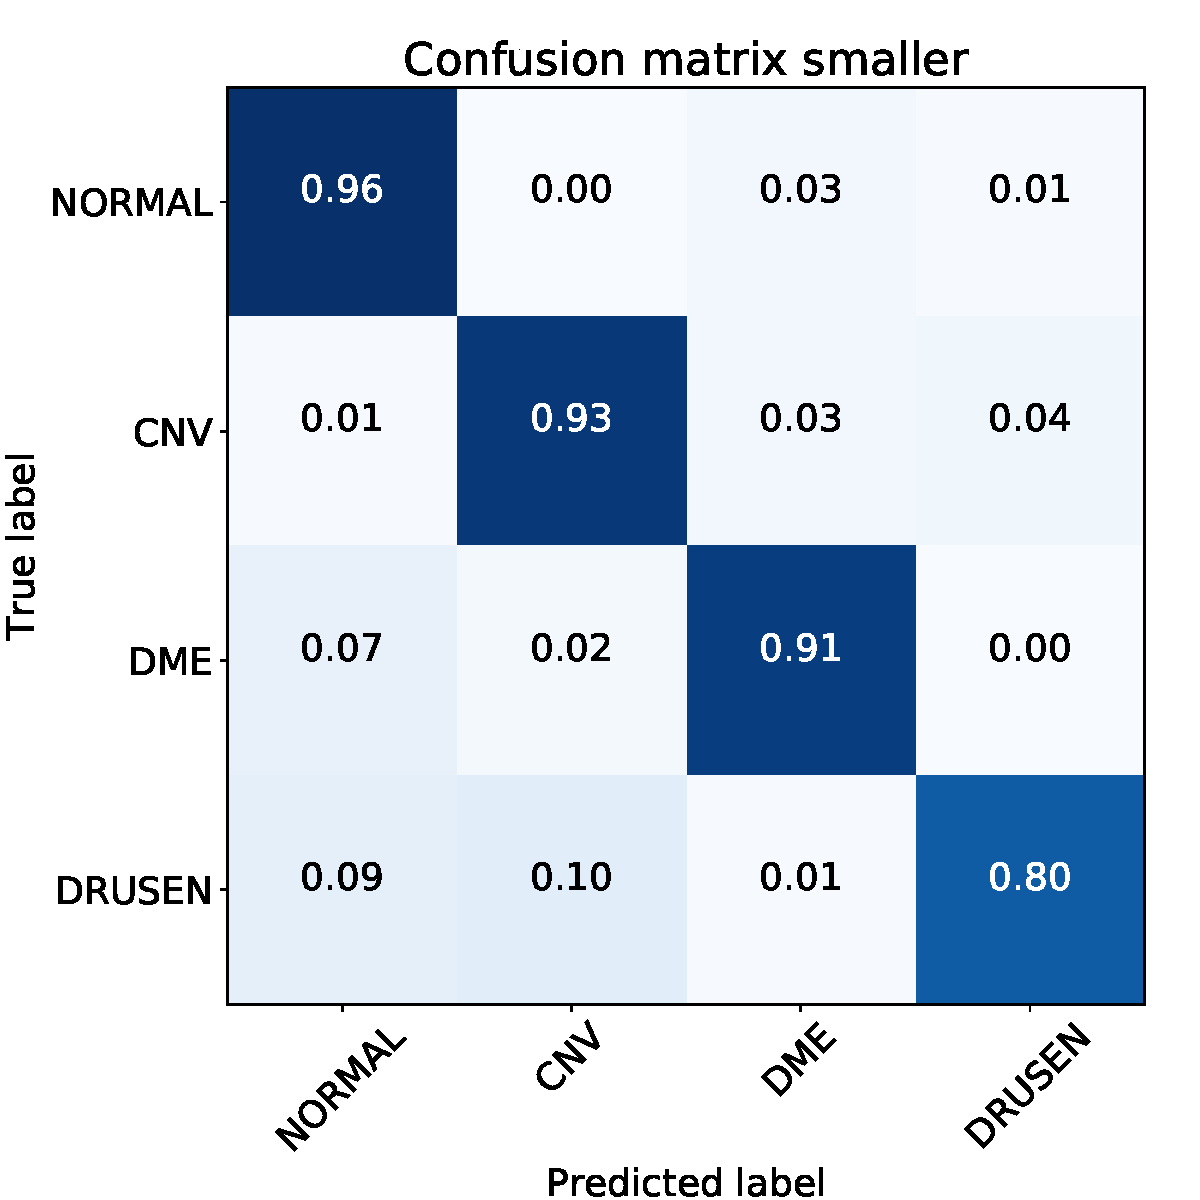
\includegraphics[width=0.4\textwidth]{Plots/confusion_matrix_smaller.pdf}}
  \hspace{8pt}
  \subcaptionbox{\label{fig:ug}}{\centering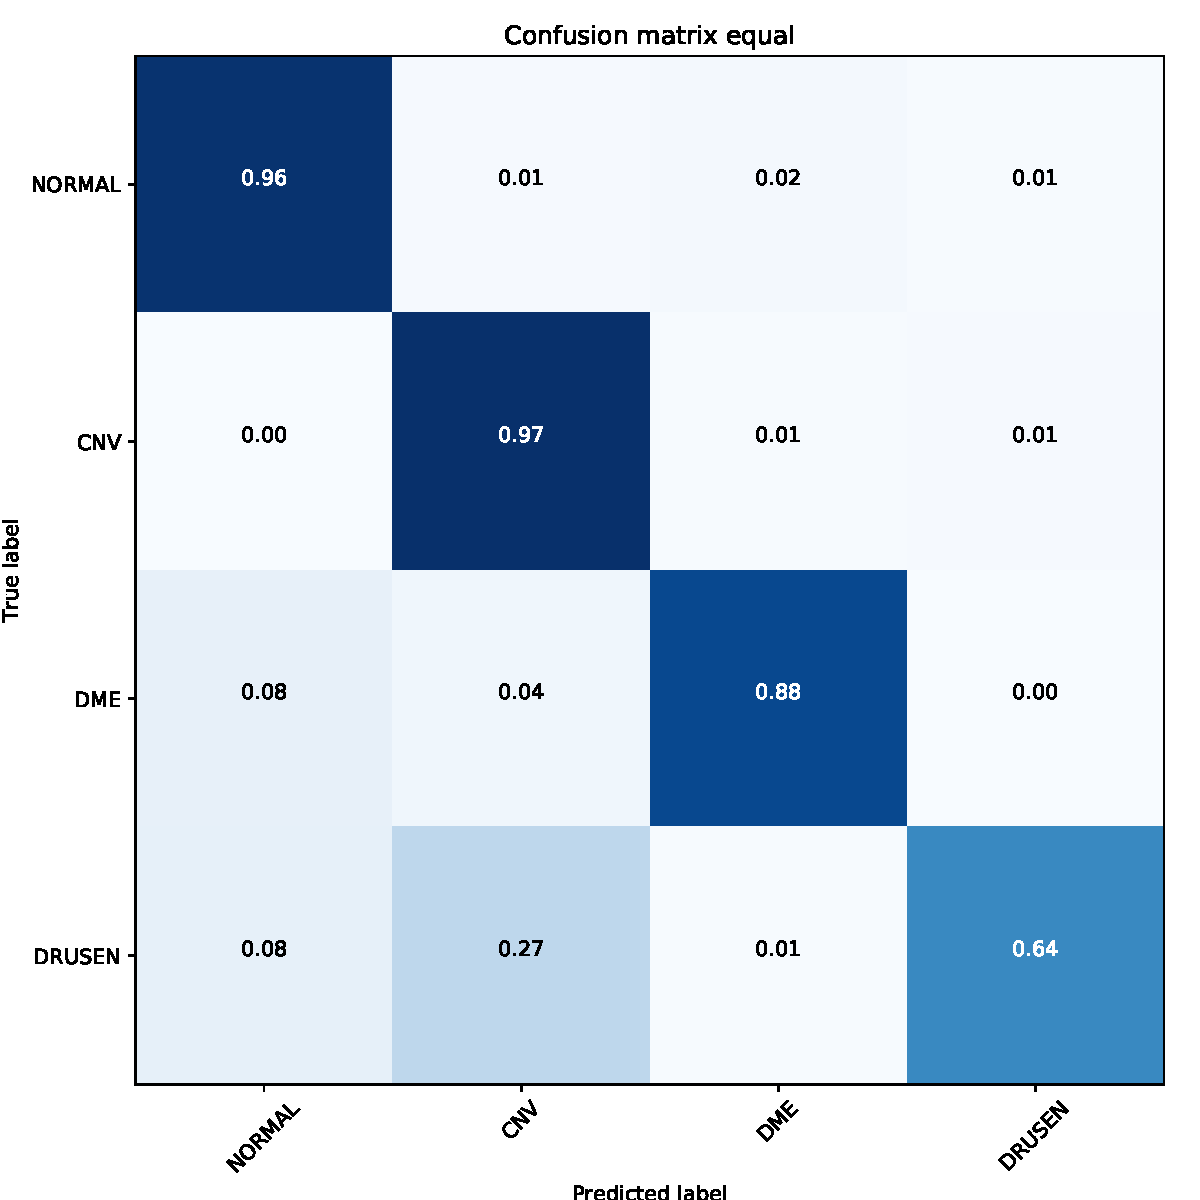
\includegraphics[width=0.4\textwidth]{Plots/confusion_matrix_equal.pdf}}
  \caption{Die Verwirrungsmatrix für das gewichtete \protect\subref{fig:g} und das ungewichtete Training \protect\subref{fig:ug}.}\label{fig:eq_all}
\end{figure}
%
Ein Netz, welches einwandfrei alle Klassen erkennen kann würde eine
Diagonalmatrix liefern. Allerdings zeugt auch eine diagonal-dominante Matrix
von einer gut funktionierenden Trennung. In diesem Falle sind die Einträge der
Matrix auf die Gesamtzahl der Bilder jeder wahren Klasse normiert, sodass die
Diagonaleinträge direkt die Genauigkeit für die explizite Klasse angeben.
Hierbei zeigt sich klar, dass bei dem ungewichteten Training wie erwartet die
Genauigkeiten für die Klassen mit vielen Bildern stark zunimmt, während die
kleinste Klasse (hier DRUSEN) am schlechtesten erkannt wird. Um dennoch von
einem möglichst großen Datensatz zu profitieren, wurde das Modell mit dem
gesamten Datensatz gewichtet trainiert.
%
\begin{figure}[h!]
  \subcaptionbox{DME}{\centering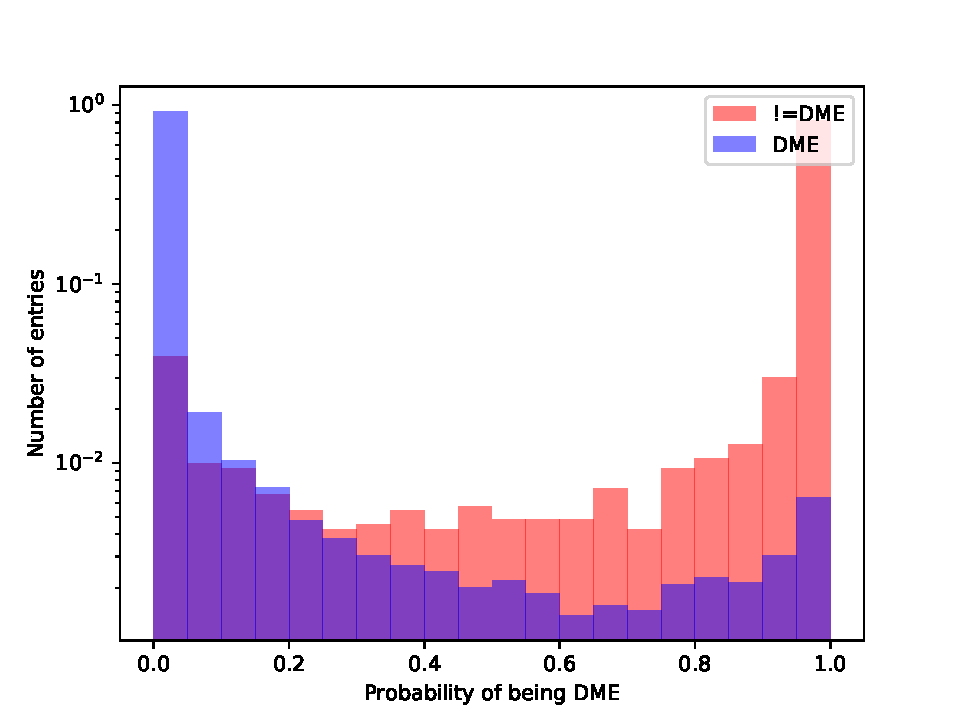
\includegraphics[width=0.48\linewidth]{Plots/DME_or_not_log_smaller.pdf}}
  \hspace{8pt}
  \subcaptionbox{CNV}{\centering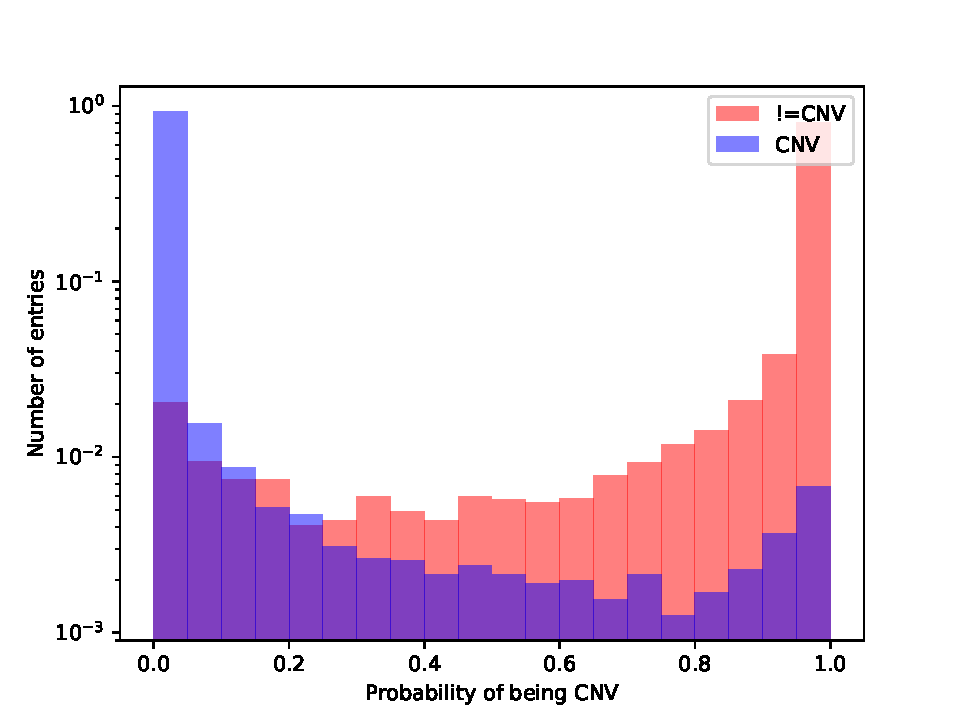
\includegraphics[width=0.48\linewidth]{Plots/CNV_or_not_log_smaller.pdf}}
  \subcaptionbox{DRUSEN}{\centering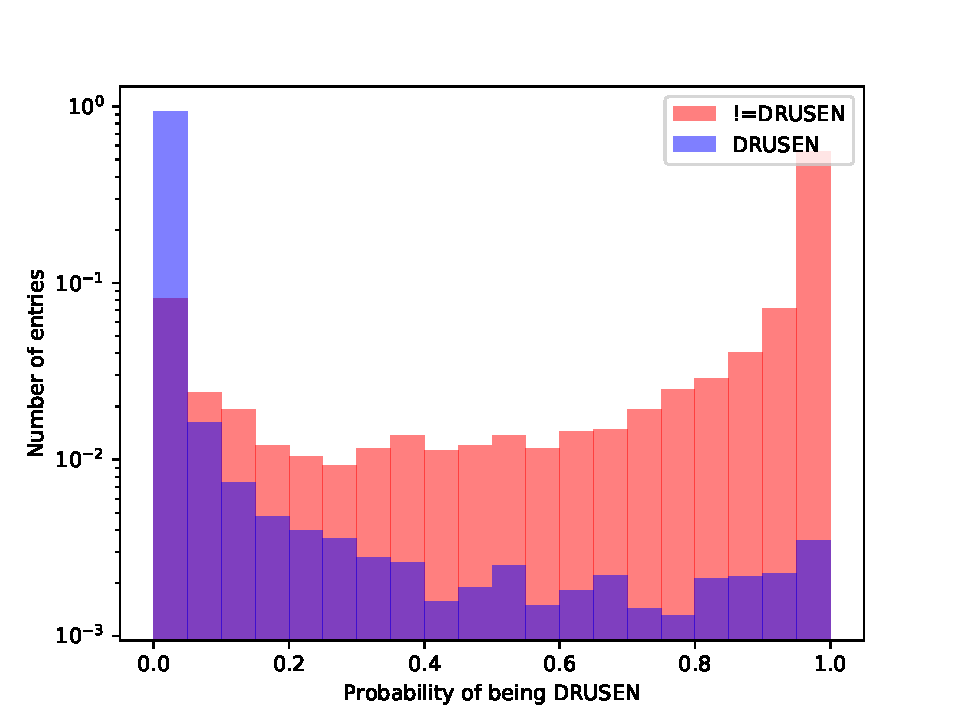
\includegraphics[width=0.48\linewidth]{Plots/DRUSEN_or_not_log_smaller.pdf}}
  \hspace{8pt}
  \subcaptionbox{NORMAL}{\centering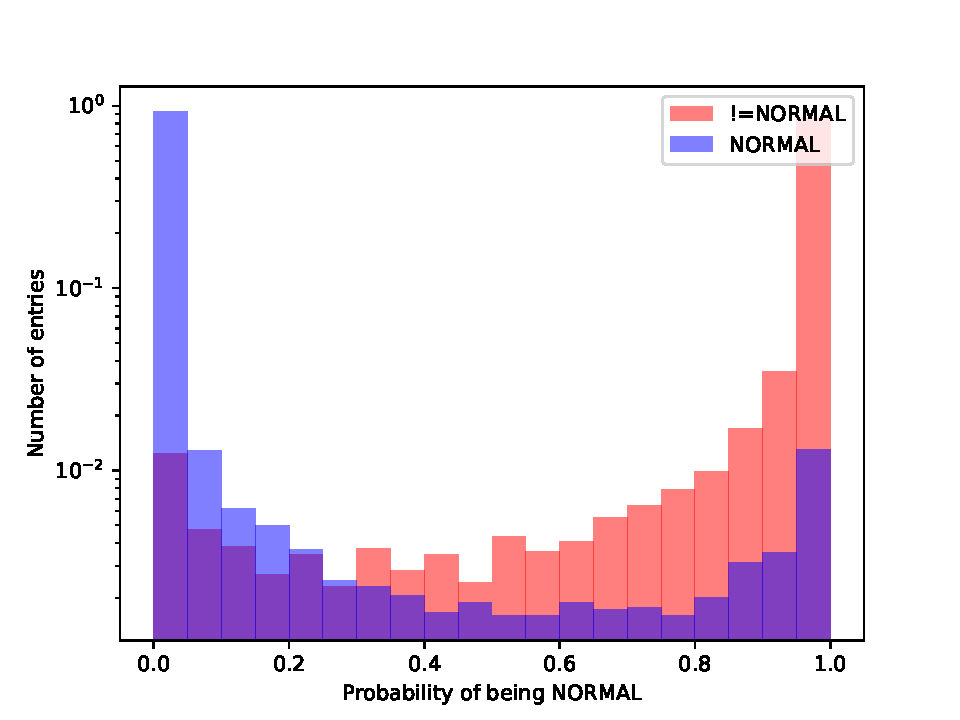
\includegraphics[width=0.48\linewidth]{Plots/NORMAL_or_not_log_smaller.pdf}}
  \caption{Ausgabe des Netzes für Bilder der einzelnen Klassen (normiert auf die Gesamtzahl der Klasse). Durch die softmax Funktion kann der Ausgabewert als Wahrscheinlichkeit für die Angehörigkeit zu einer Klasse interpretiert werden. Zwei Bins der Höhe 1 bei 0 und 1 würden eine perfekte Trennung repräsentieren.}
\end{figure}
%

\chapter{Alternative Methode}

Als alternative Methode zur Klassifizierung der 4 Klassen wird ebenfalls ein
neuronales Netz verwendet. Es erwies sich als äußerst schwierig, für diese
Problemstellung einen Lösungsansatz zu finden, der auf die Verwendung
neuronaler Netze verzichten kann. Wie zu Beginn dieser Arbeit bereits erwähnt,
gehört dieser Aufgabentyp zu den Aufgaben, die für Computer mit herkömmlichen
Methoden schwierig zu lösen sind.
Wie in Abschnitt~\ref{sec:netze} bereits beschrieben, eignen sich CNN am besten
zur Bilderkennung. Die Alternativmethode soll eine deutlich einfachere Lösung
darstellen, die einerseits zeigen soll, ob eine Lösung des Problems so möglich
ist und damit andererseits die \textit{performance} der Hauptarchitektur
relativieren. Daher verzichtet die Alternativmethode gänzlich auf CNN.
Außerdem wird der Datensatz so weit herunterskaliert, dass das Training auf
einem herkömmlichen PC in vertretbarer Rechenzeit durchgeführt werden kann.
%
\begin{figure}[h!]
  \subcaptionbox{Auf eine Größe von $50\text{px}\times100\text{px}$ skaliertes Beispielbild.}{\centering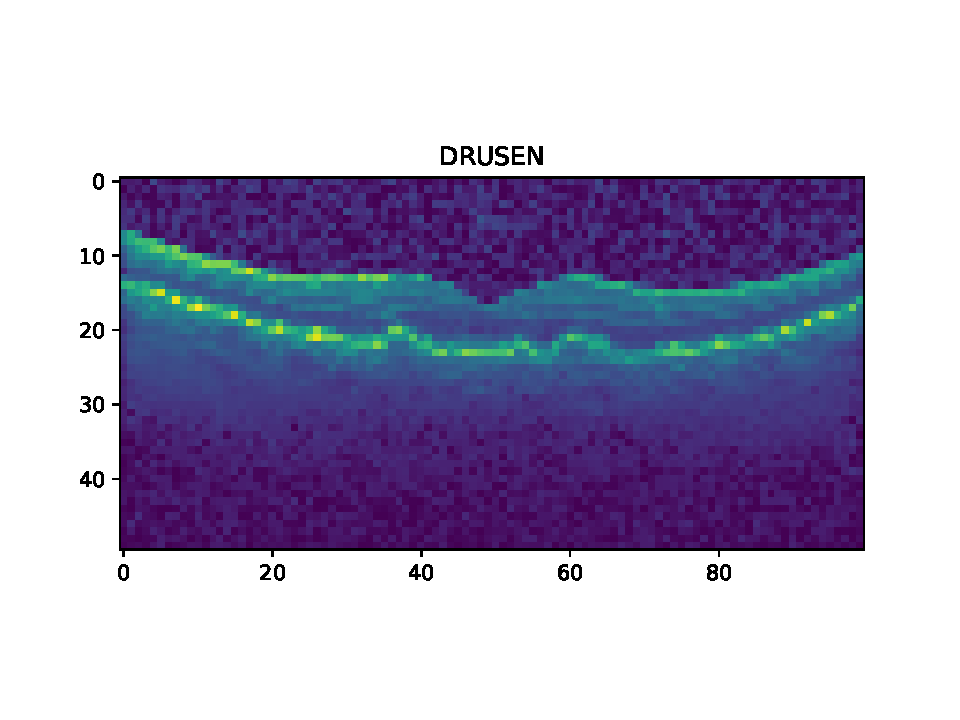
\includegraphics[width=0.5\linewidth]{Plots/image_0.pdf}}
  \hspace{5pt}
  \subcaptionbox{Die Verteilung der Mittelwerte aus dem \textit{Pooling} dieses Bildes.}{\centering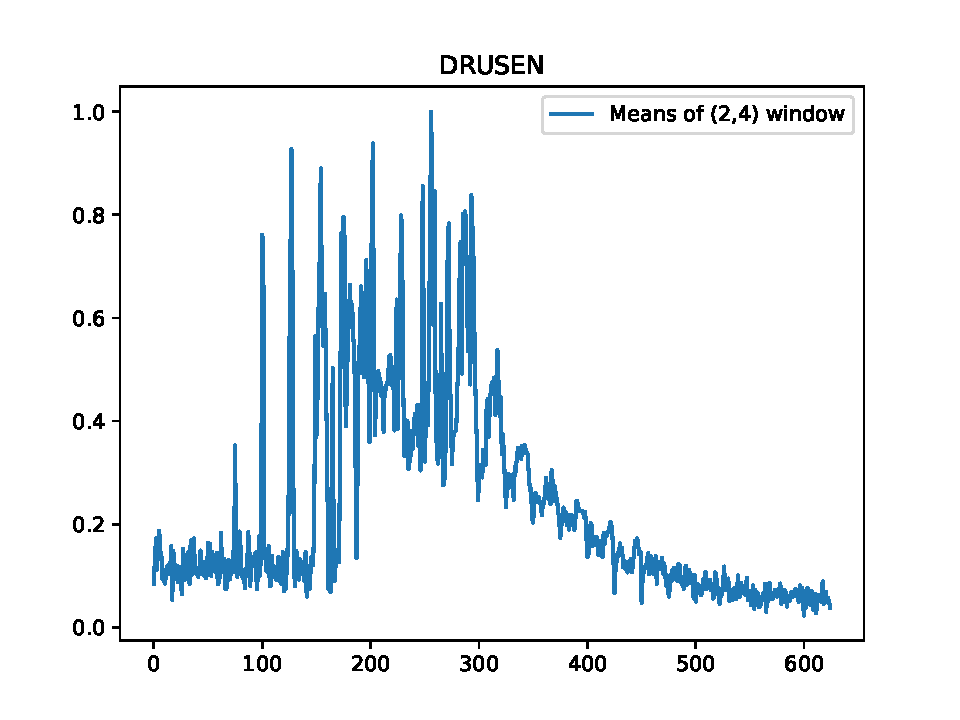
\includegraphics[width=0.5\linewidth]{Plots/distr.pdf}}
  \caption{Veranschaulichung der Datenskalierung für die Alternativmethode. Die Bilder werden zugeschnitten, skaliert und einem \textit{AveragePooling} unterzogen.}
  \label{fig:alter}
\end{figure}
%
Für diese Methode haben wir es uns zu Nutze gemacht, dass das Erkennen der
Krankheiten hauptsächlich im Bildmittelpunkt stattfindet. Die OCT Aufnahmen
sind verständlicherweise auf die Iris zentriert aufgenommen.
Daher wird das Bild zunächst zugeschnitten. Dazu werden die Pixelwerte auf eine
Achse projiziert, indem zeilenweise aufsummiert wird. In dieser Verteilung
lässt sich ein Maximum finden, welches als Mittelpunkt des Bildes dient.
Von diesem Mittelpunkt aus wird das Bild auf eine Größe von lediglich
$50\text{px}\times100\text{px}$ zugeschnitten. Dies reduziert die Dateigröße
und damit auch die Anzahl der \textit{input features} bereits etwa um einen
Faktor $30$.
Das so entstandene Bild wird schließlich einem \textit{Pooling} unterzogen.
Dazu wird in einem Fenster aus $2\times4$ Pixeln der Mittelwert berechnet und
dieser einzelne Wert als Input gespeichert. Das Verfahren ist in
Abbildung~\ref{fig:alter} veranschaulicht. \\
Der so generierte Datensatz wird dann einem \textit{fully connected} Netz aus
Dichtelagen zum Training bereitgestellt. Die Architektur dieses Netzes ist in
XXX dargestellt.\\
Es handelt sich hierbei um ...\\
Die hierzu verwendete Architektur ist das Ergebnis einer intensiven
\textit{grid search}. Durch die Skalierung des Datensatzes und die Verwendung
eines deutlich kleineren Netzes kann die Rechenzeit für das Training eines
Netzes stark reduziert werden. Dies ermöglicht auch eine intensive Suche nach
der besten Hyperparameterkonfiguration. Dazu wurden die Anzahl der Dichtelagen
in Kombination mit der Anzahl der Filter der einzelnen Dichtelagen, die
Aktivierungsfunktion in den Dichtelagen, sowie die Aktivierungsfunktion der
letzten Lage, sowie die Raten für die \textit{Dropout} Lagen variiert. So
konnten insgesamt mehr als $120$ Modellarchitekturen getestet werden. Die
Architektur mit der höchsten \textit{performance} ist oben beschrieben.

\chapter{Ergebnisse}

Die Klassifizierung des Zustandes der menschlichen Retina anhand von OCT
Aufnahmen in 4 Klassen (gesund + 3 Erkrankungen) lässt sich mit Hilfe des
maschinellen Lernens mit einer Genauigkeit von bis zu $\SI{90}{\percent}$
durchführen. Eine Lösung dieser Aufgabe, wie sie in dieser Arbeit beschrieben
ist, erfordert allerdings eine sehr hohe Rechenkapazität. Der verwendete
Datensatz liefert mit etwa $90\,000$ Bildern in sehr guter Auflösung eine
ausreichende Statistik, um gute Ergebnisse zu erzielen.
Die Hauptarchitektur eines CNN zeigt hierbei mit Abstand die beste
Genauigkeit. Nach etwa 40 Epochen lässt sich mit diesem Netz ein
Modell generieren, welches 4 Klassen mit einer Genauigkeit von
$\SI{90}{\percent}$ unterscheiden kann. Durch die Architektur können so Bilder
verschiedener Größen und Datensätze unterschiedlicher Verteilungen zur
Vorhersage verwendet werden. Durch ausreichende Regularisierung treten keine
Effekte von Übertraining auf, wie in Abbildung~\ref{fig:hist} zu sehen
ist.
%
\begin{figure}[h!]
  \subcaptionbox{Genauigkeit\label{fig:gen}}{\centering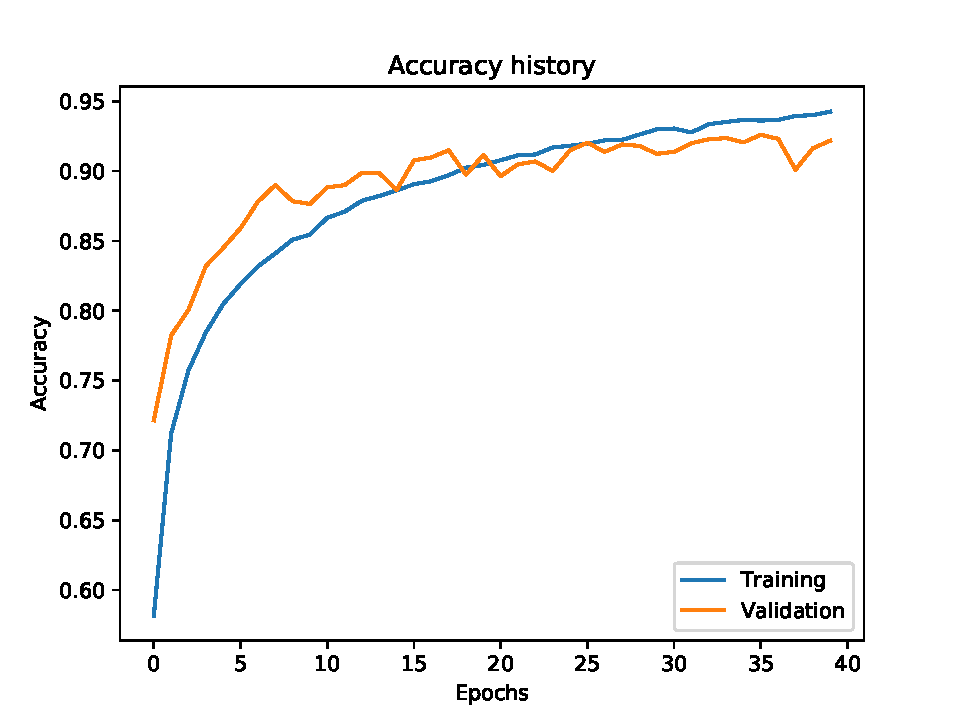
\includegraphics[width=0.5\linewidth]{Plots/accuracy_history_smaller.pdf}}
  \subcaptionbox{Verlustfunktion\label{fig:lo}}{\centering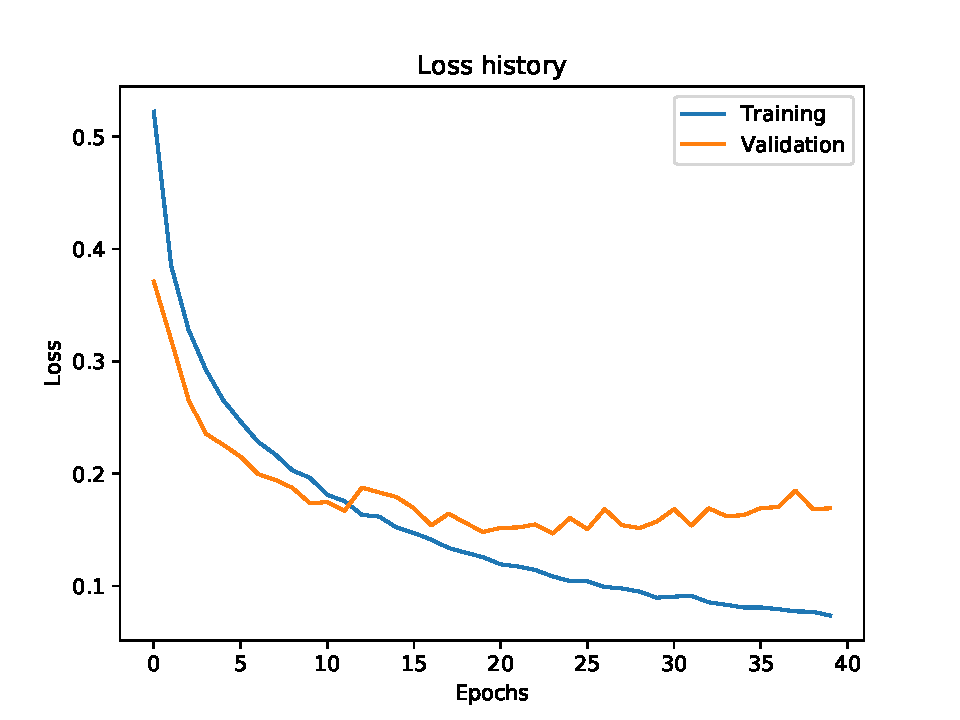
\includegraphics[width=0.5\linewidth]{Plots/loss_history_smaller.pdf}}
  \caption{Die Genauigkeit \protect\subref{fig:gen}, sowie die Verlustfunktion \protect\subref{fig:lo} der Hauptarchitektur des CNN. Es zeigen sich hier nach 40 Epochen keine Anzeichen für ein \textit{overtraining}.}
  \label{fig:hist}
\end{figure}
%
Betrachtet man Beispiele für die Klassen CNV, DRUSEN und NORMAL, deren
Trennung für das Netz am schwierigsten ist, so fällt auf, dass es sich hierbei
um Bilder handelt, die auch für Menschen schwierig zu trennen sind. Das Netz
erreicht allerdings mit der oben beschriebenen Genauigkeit eine Präzesion, die
weit über der eines ungelernten Auges liegt. Ärzte hingegen erreichen
Genauigkeiten, die noch über dem hier erreichten Wert liegen.\\
Eine Genauigkeit von $\SI{90}{\percent}$ durch Bilderkennung auf 4 Klassen zu
erreichen, stellt allerdings eine sehr optimistisch stimmende Leistung dar.
Ein Vergleich mit der Genauigkeit der Diagnose der Erkrankung CNV durch
Mediziner zeigt, dass die hier erreichten $\SI{93}{\percent}$ über der in einer
Studie~\cite{CNV} erreichten Genauigkeit von $\SI{86.5}{\percent}$ liegen.
\newpage
%
\begin{figure}[h!]
  \subcaptionbox{Verwirrungsmatrix\label{fig:conf}}{\centering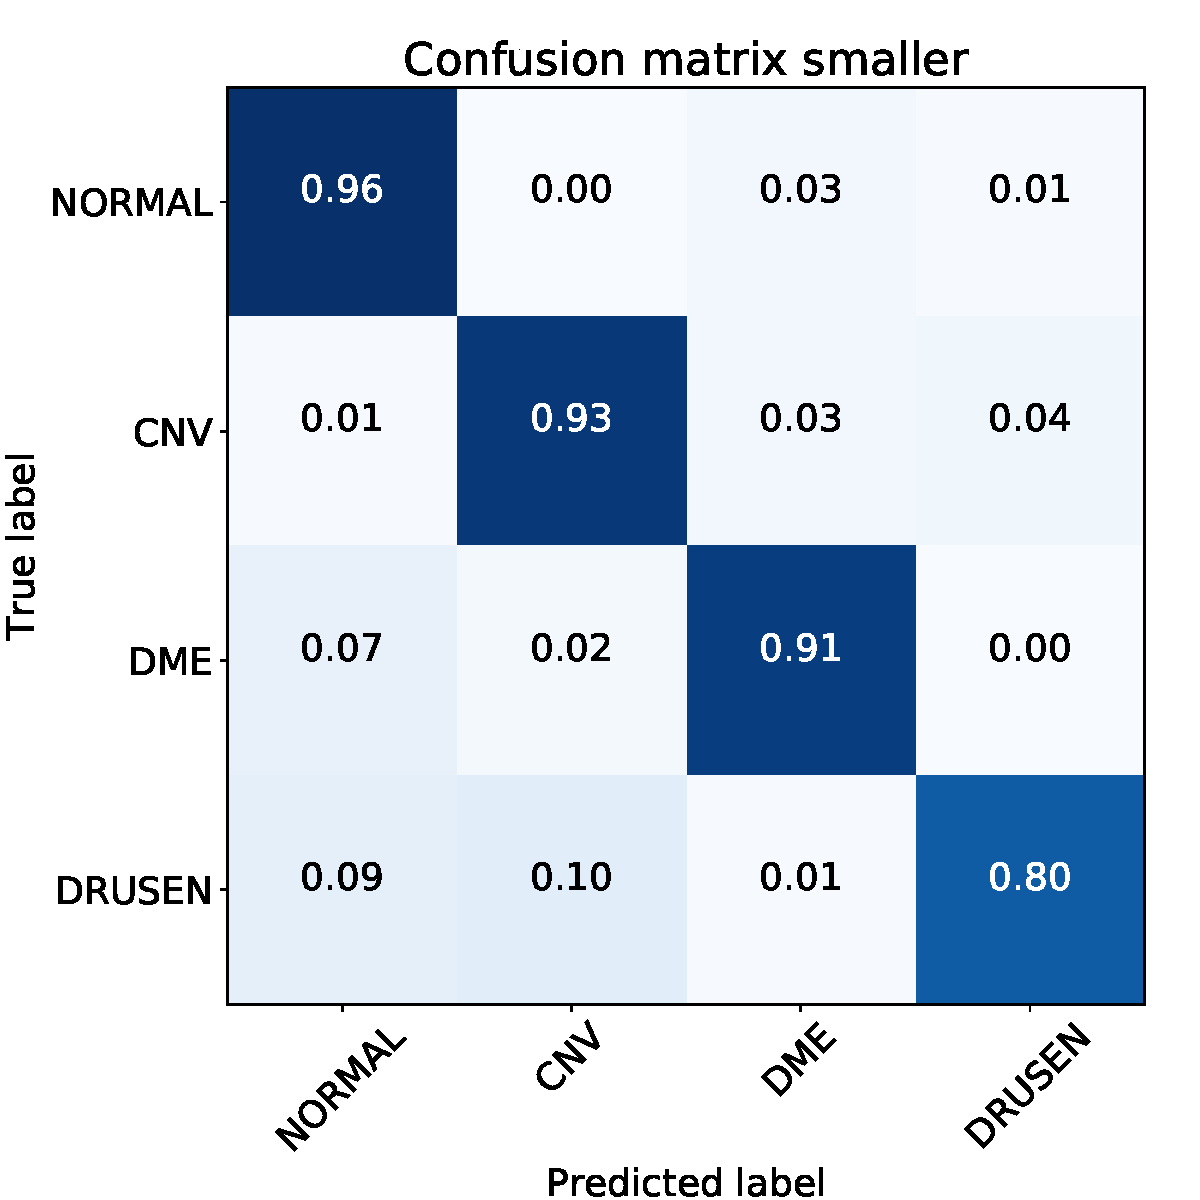
\includegraphics[width=0.4\linewidth]{Plots/confusion_matrix_smaller.pdf}}
  \subcaptionbox{Verteilung des Outputs des Netzes für ein Validierungssample\label{fig:out}}{\centering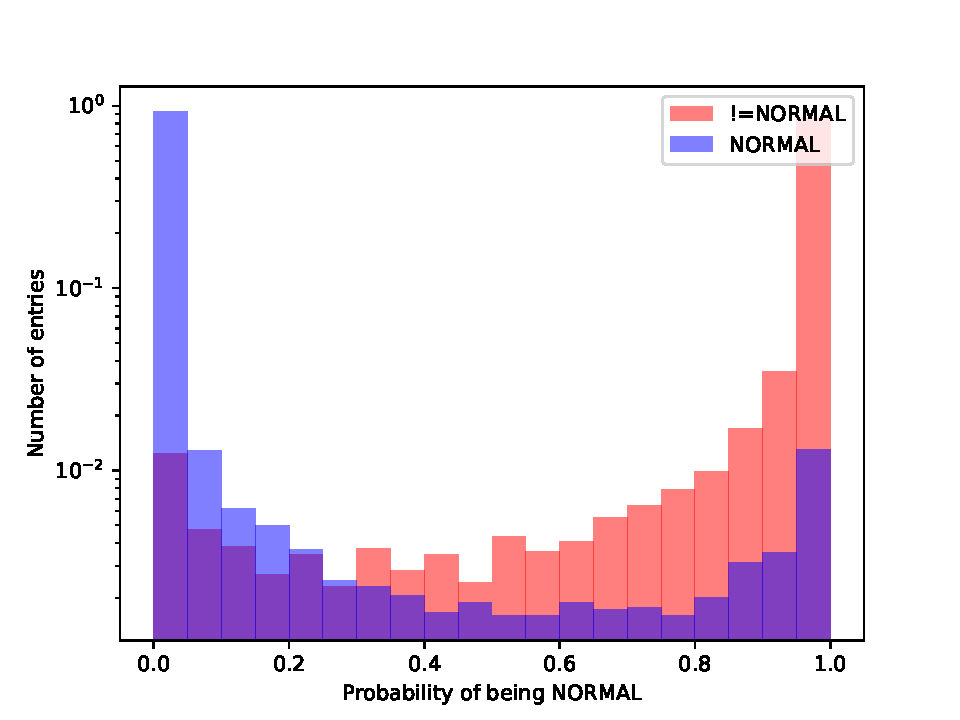
\includegraphics[width=0.55\linewidth]{Plots/NORMAL_or_not_log_smaller.pdf}}
  \caption{Die Verwirrungsmatrix \protect\subref{fig:conf}, sowie der Output \protect\subref{fig:out} der Hauptarchitektur des CNN. Die Verwirrungsmatrix zeigt sehr hohe Genauigkeiten für die einzelnen Klassen. Der Output des Netzes zeigt ebenfalls eine gute Trennung der Krankheiten vom gesunden Auge.}
  \label{fig:erg}
\end{figure}
%
Allerdings zeigt diese Arbeit auch, dass sich mit deutlich einfacheren
Architekturen funktionierende Modelle entwickeln lassen, deren Genauigkeit weit
über dem Zufall liegen. Insbesondere zeigt sich trotz starker Skalierung des
Datensatzes, was eine deutliche Verringerung der Rechenzeit
zur Folge hat, eine Lösung mit einem einfachen vollständig vernetzten Netz.
Dabei ist eine Genauigkeit von etwa $\SI{73}{\percent}$ möglich. Dies liegt
deutlich unterhalb dessen, was das CNN leisten kann und zeigt damit auch, dass
CNN auf diesem Datensatz deutlich effektiver sind. Die damit erreichten
$\SI{90}{\percent}$ Genauigkeit stellen damit ein sehr gutes Ergebnis dar.
%
\begin{figure}[h!]
  \subcaptionbox{Verwirrungsmatrix\label{fig:conf_alt}}{\centering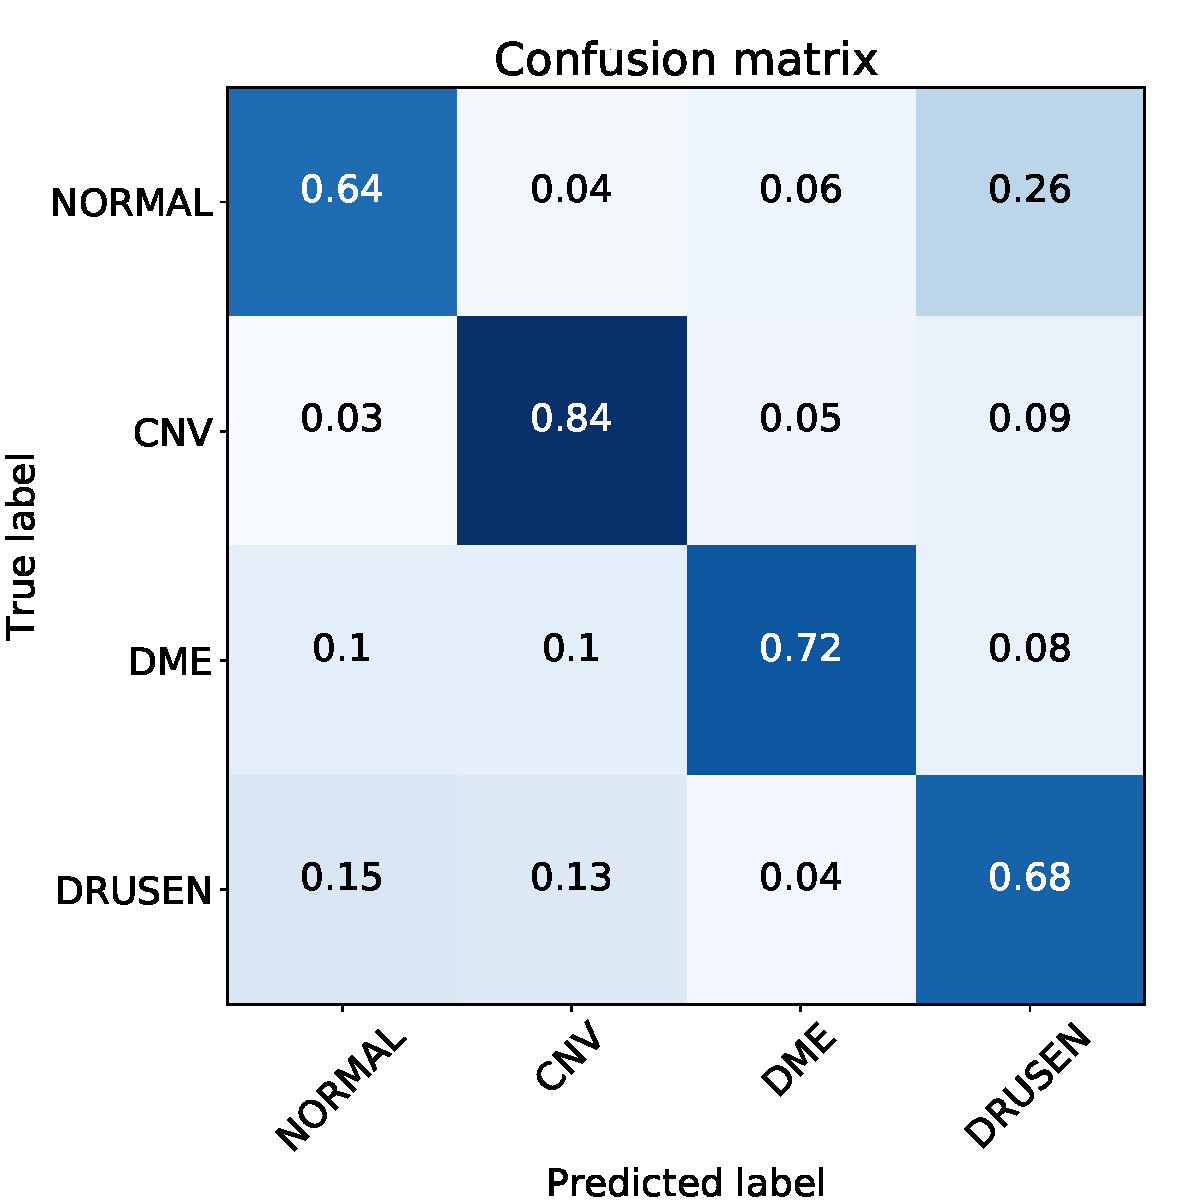
\includegraphics[width=0.4\linewidth]{Plots/confusionmatrix6test.pdf}}
  \subcaptionbox{Verlauf der Genauigkeit\label{fig:acc_alt}}{\centering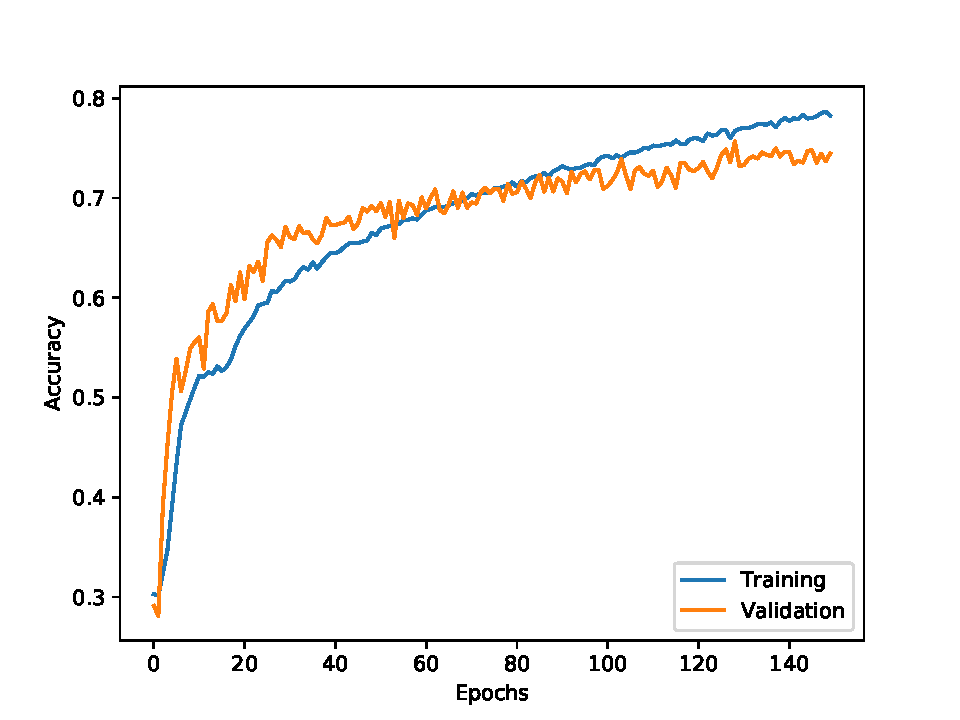
\includegraphics[width=0.55\linewidth]{Plots/accuracyhistory6.pdf}}
  \caption{Die Verwirrungsmatrix \protect\subref{fig:conf_alt}, sowie der Verlauf der Genauigkeit \protect\subref{fig:acc_alt} während des Trainings der Alternativmethode. Die Verwirrungsmatrix zeigt deutlich geringere Genauigkeiten als das CNN. Der Verlauf der Genauigkeit zeigt, dass ein längeres Trainieren ins overtraining führt.}
  \label{fig:erg}
\end{figure}
%
Auch für die Alternativmethode zeigt sich in Abbildung~\ref{fig:conf}, dass die
Unterscheidung der Klasse DRUSEN von den Klassen NORMAL und CNV besonders
schwierig erscheint. Allerdings scheint die Präparation der Daten wie in
Abschnitt~\ref{sec:alter} beschrieben, dafür zu sorgen, dass insbesondere auch
gesunde Retinas in etwa $\SI{25}{\percent}$ der Fälle für DRUSEN gehalten
werden.


\appendix
% Hier beginnt der Anhang, nummeriert in lateinischen Buchstaben
\chapter{Ein Anhangskapitel}

Hier könnte ein Anhang stehen, falls Sie z.B. Code, Konstruktionszeichnungen oder Ähnliches mit in die Arbeit bringen wollen. Im Normalfall stehen jedoch alle Ihre Resultate im Hauptteil der Bachelorarbeit und ein Anhang ist überflüssig.


\backmatter
\printbibliography

% \cleardoublepage
% \thispagestyle{empty}
\section*{Eidesstattliche Versicherung}
Ich versichere hiermit an Eides statt, dass ich die vorliegende Abschlussarbeit mit dem Titel \enquote{\thetitle} selbstständig und ohne unzulässige fremde Hilfe erbracht habe.
Ich habe keine anderen als die angegebenen Quellen und Hilfsmittel benutzt, sowie wörtliche und sinngemäße Zitate kenntlich gemacht. 
Die Arbeit hat in gleicher oder ähnlicher Form noch keiner Prüfungsbehörde vorgelegen.

\vspace*{1cm}\noindent
\begin{center}
  \begin{tabular}{@{}p{0.4\textwidth}@{\hspace{0.15\textwidth}}p{0.4\textwidth}@{}}
  \rule{\linewidth}{0.25pt}& \rule{\linewidth}{0.25pt}\\
  Ort, Datum & Unterschrift
  \end{tabular}
\end{center}

\subsection*{Belehrung}
Wer vorsätzlich gegen eine die Täuschung über Prüfungsleistungen betreffende Regelung einer Hochschulprüfungsordnung verstößt, handelt ordnungswidrig.
Die Ordnungswidrigkeit kann mit einer Geldbuße von bis zu \SI[round-mode=places, round-precision=2]{50000}{€} geahndet werden. 
Zuständige Verwaltungsbehörde für die Verfolgung und Ahndung von Ordnungswidrigkeiten ist der Kanzler/die Kanzlerin der Technischen Universität Dortmund. 
Im Falle eines mehrfachen oder sonstigen schwerwiegenden Täuschungsversuches kann der Prüfling zudem exmatrikuliert werden \mbox{(\S\,63 Abs. 5 Hochschulgesetz --HG--).}

Die Abgabe einer falschen Versicherung an Eides statt wird mit Freiheitsstrafe bis zu 3 Jahren oder mit Geldstrafe bestraft.

Die Technische Universität Dortmund wird ggf.\ elektronische Vergleichswerkzeuge (wie z.\,B.\ die Software \enquote{turnitin}) zur Überprüfung von Ordnungswidrigkeiten in Prüfungsverfahren nutzen. \\[\baselineskip]

\noindent Die oben stehende Belehrung habe ich zur Kenntnis genommen.\\[1cm]
\begin{center}
\begin{tabular}{@{}p{0.4\textwidth}@{\hspace{0.15\textwidth}}p{0.4\textwidth}@{}}
\rule{\linewidth}{0.25pt}& \rule{\linewidth}{0.25pt}\\
Ort, Datum & Unterschrift
\end{tabular}
\end{center}

\end{document}
